%% LyX 2.0.2 created this file.  For more info, see http://www.lyx.org/. 
%% Do not edit unless you really know what you are doing.
\documentclass[english,review]{acmsiggraph}
\usepackage[T1]{fontenc}
\usepackage[latin9]{inputenc}
\usepackage{amssymb}
\usepackage{graphicx}

\makeatletter
%%%%%%%%%%%%%%%%%%%%%%%%%%%%%% User specified LaTeX commands.
% for the following cases use the listed document class option:
% [annual] - Technical paper accepted for presentation at the ACM SIGGRAPH 
%   or SIGGRAPH Asia annual conference.
% [sponsored] - Short or full-length technical paper accepted for 
%   presentation at an event sponsored by ACM SIGGRAPH
%   (but not the annual conference Technical Papers program).
% [abstract] - A one-page abstract of your accepted content
%   (Technical Sketches, Posters, Emerging Technologies, etc.). 
%   Content greater than one page in length should use the "[sponsored]"
%   parameter.
% [preprint] - A preprint version of your final content.
% [review] - A technical paper submitted for review. Includes line
%   numbers and anonymization of author and affiliation information.

% When you submit your paper for review, please use the \TOGonlineID''
% command to include the online ID value assigned to your paper by the
% submission management system. Replace '45678' with the value you were
% assigned.
\TOGonlineid{XXXXX}

% If you are preparing a preprint of your accepted paper, and your paper
% will be published in an issue of the ACM "Transactions on Graphics''
% journal, replace the "0'' values in the commands below with the correct
% volume and number values for that issue - you'll get them before your
% final paper is due.
\TOGvolume{0}
\TOGnumber{0}

% The TOGarticleDOI' command accepts the DOI information provided to you
% during production, and which makes up the URLs which identifies the ACM
% article page and direct PDF link in the ACM Digital Library.
% Replace "1111111.2222222'' with the values you are given.
\TOGarticleDOI{1111111.2222222}

% If you would like to include links to personal repositories for auxiliary
% material related your research contribution, you may use one or more of
% these commands to define an appropriate URL. The "\TOGlinkslist'' command
% found just before the first section of your document will add hyperlinked
% icons to your document, in addition to hyperlinked icons which point to
% the ACM Digital Library article page and the ACM Digital Library-held PDF.
\TOGprojectURL{}
\TOGvideoURL{}
\TOGdataURL{}
\TOGcodeURL{}

% Paper title.
\title{Curvature Enhance With and Adapted Laplacian Operator For Hybrid Quad/Triangle Meshes}

% Author and Affiliation (single author).
%\author{Name \thanks{e-mail: name@unknown.uu}\\ Research Institute}

% Author and Affiliation (multiple authors).
\author{Alexander Pinzon\thanks{e-mail: apinzonf@gmail.com}
\qquad  Eduardo Romero\thanks{e-mail:edromero@unal.edu.co}
 \\Cimalab Research Group\\National University of Colombia}
%\and Ton Roosendaal\thanks{e-mail:ton@blender.org}\\ Blender CEO}

% The ``pdfauthor'' command accepts the authors of the work,
% comma-delimited, and adds this information to the PDF metadata.
%\pdfauthor{Alexander Pinzon, Eduardo Romero, Ton Roosendaal}
\pdfauthor{Anonymous}

% Keywords that describe your work.
\keywords{laplacian smooth, curvature, sculpting, subdivision surface}

\makeatother

\usepackage{babel}
\begin{document}







\teaser{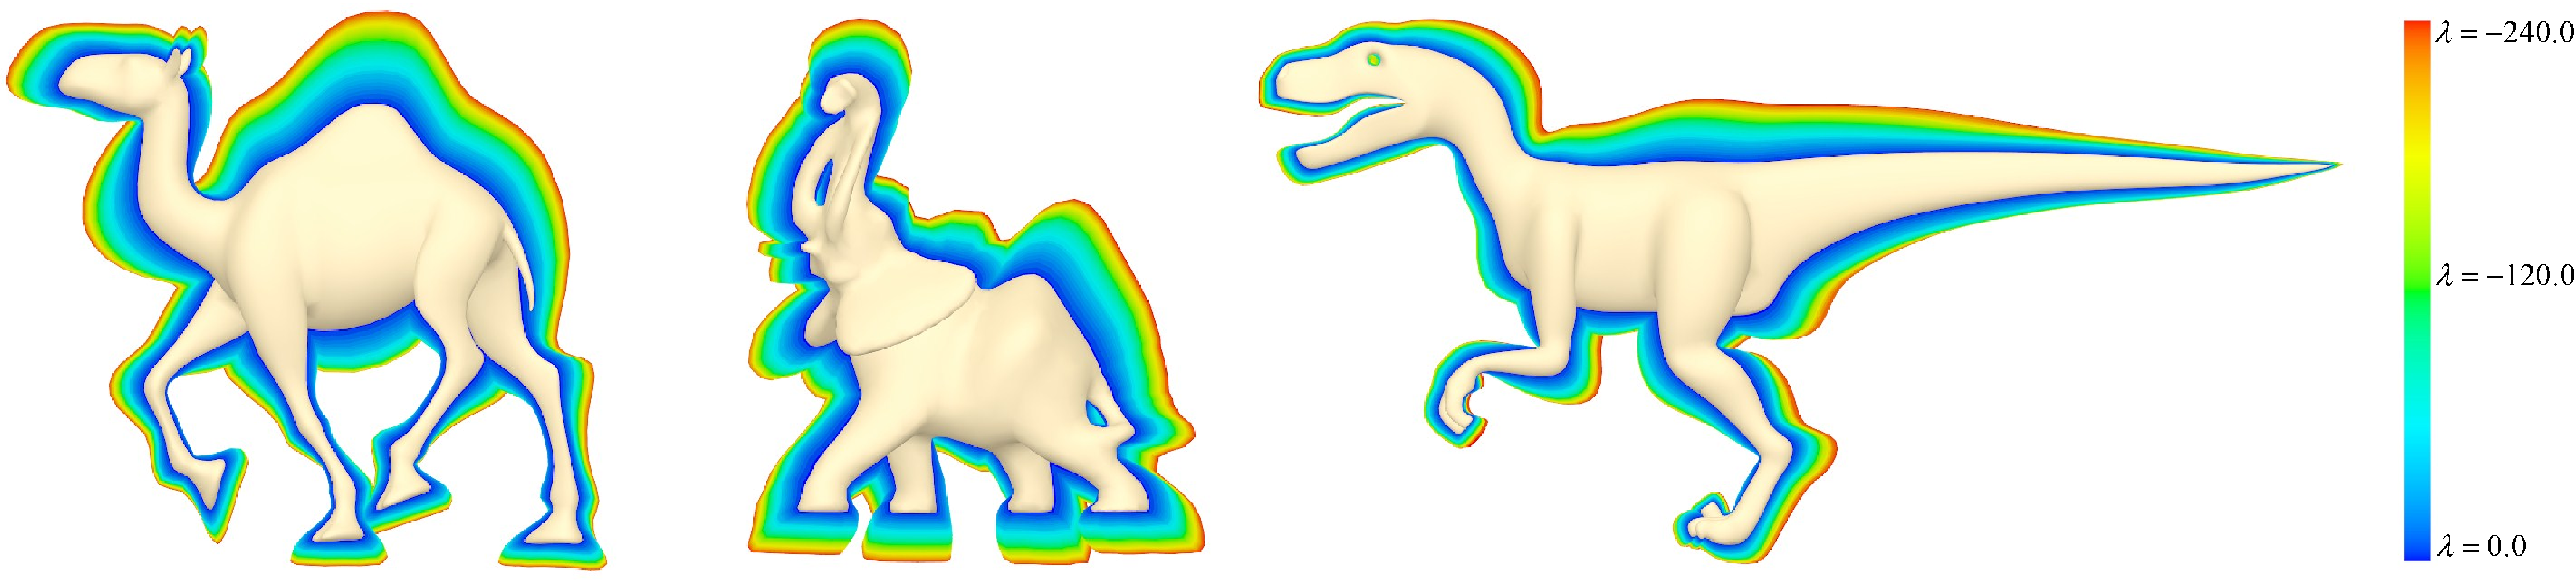
\includegraphics[width=1\textwidth]{images/spectrum} \caption{\label{fig:Spectrum}A set of 48 successive curvature enhance shapes,
from $\lambda=0.0$ in blue to $\lambda=-240.0$ in red, with steps
of $-5.0$.}
}

\maketitle
\maketitle 
\begin{abstract}
This paper proposes a novel method for modeling a polygonal mesh by
enhancing the object curvature. This method uses an adapted extension
of the Laplace Beltrami operator for hybrid quad/triangle meshes,
to enhance the global curvature. Along with the method, this work
also presents new applications of curvature enhancement in sculpting
and modeling with subdivision surfaces and weight vertex groups. A
series of graphics examples demonstrates the quality, predictability
and flexibility of the method in a real production environment with
software blender.
\end{abstract}

\begin{CRcatlist}
\CRcat{I.3.5}{Computer Graphics}{Computational Geometry and Object Modeling
}{Modeling packages}
\end{CRcatlist}
\keywordlist

\TOGlinkslist

%\copyrightspace


\section{Introduction}

Over the last years several modeling techniques have been developed
to generate a variety of shapes that look natural and realistic\cite{Botsch2006}.
Editing techniques have evolved from affine transformations to advanced
tools like sculpting \cite{Coquillart1990,Galyean1991,Stanculescu2011},
editing and creation from sketches \cite{Igarashi1999,Gonen2012},
and complex interpolation techniques \cite{Sorkine2004,Zhou2005}.

Traditional methods for smoothing surfaces from coarse geometry, like
the Catmull-Clark, have become widely popular \cite{Catmull1978,Stam1998}.
These works generalize the uniform B-cubic splines knot insertion
to meshes, some of them adding some type of control, for instance
with the use of creases to produce sharp edges \cite{DeRose1998},
or the modification of weights on the vertices to locally control
the zone of influence \cite{Biermann2000}. Instead, the presented
method performs a feature enhancement of the model by parameterizing
the surface curvature and thereby creating a family of different versions
of the same object, preserving therefore the detail of the original
model and a realistic appearance. 

On the other hand, many types of brushes have been developed to sculpt
meshes. Brushes that perform inflation end up by losing detail when
inflating the vertices \cite{Stanculescu2011}, in contrast the presented
method allows inflation of the mesh vertices by moving them towards
the opposite curvature direction, conserving the shape and sharp features
of the model.

\textbf{Contributions} This work presents an extension of the Laplace
Beltrami operator for hybrid quad/triangle meshes representing a larger
mesh spectrum from what has been presented so far. The method eliminates
the need of preprocessing and allows preservation of the original
topology. Likewise, along with this operator, it is proposed a method
to generate a family of parameterized shapes, in a robust and predictable
way. This method enables customization of the smoothness and curvature,
obtained during the subdivision surfaces process. Finally, it is proposed
a new brush for enhancing silhouette mesh features in modeling and
sculpting.

This work is organized as follows: Section \ref{sub:1.1-Related-work}
presents works related to the Laplacian mesh processing, digital sculpting,
and offsetting methods for polygonal meshes; In section \ref{sec:Laplacian-Smooth}
, it is described the theoretical framework of the Laplacian operator
for polygon meshes; In section \ref{sec:Proposed-Method}, it is presented
the method for curvature enhancement and applications of subdivision
of surfaces and sculpting; finally some Laplacian operator results,
to hybrid quad/triangle meshes are graphically shown as well as results
of the curvature enhancement applications in sculpting, subdivision
and modeling.


\section{Related work\label{sub:1.1-Related-work}}

Many tools have been developed for modeling, based on Laplacian mesh
processing. Thanks to the advantages of the Laplacian operator, these
different tools preserve the surface geometric details when using
them for different processes such as free-form deformation, fusion,
morphing and other application\cite{Sorkine2004}. 

Offset polygon mesh methods, based on the curvature defined by the
Laplace Beltrami operator, have been developed. These methods adjust
the shape offset by a constant distance, with high precision as to
minimize the Hausdorf error. Nevertheless, these methods fail to conserve
enough detail because of the smoothing, a crucial issue which depends
on the offset size\cite{Zhuo2012}. In volumetric approaches for point-based
representation the computing the offset boundary that are based on
distance field computation, when performing the offset, the topology
of the model may be different from the original, changing the original
design \cite{Chen2011}.

\cite{Gal2009} proposes automatic features detection and shape edition
with feature inter-relationship preservation. They define salient
surface features like ridges and valleys with based the first and
second order curvature derivatives \cite{Ohtake2004}, and angle-based
threshold. Later the curves are classified by several properties as
planar or non-planar, approximated by lines, circles, ellipses and
other complex shapes. In then the user defines an initial change over
several features and then this change is propagated over other features
with base in the classified shapes and the inter-relationships between
these. This method works fine with objects that have sharp edges composed
of basic geometric shapes such as lines, circles or ellipses but method
has problems to classify when models are smoother with organic forms
because it cannot find the features to edit and preserve.

Digital sculpting can be divided into two principal approaches: based
on polygonal methods and voxel grid-based methods. Brushes for inflate
operations in polygonal methods only depends on the normal at each
vertex \cite{Stanculescu2011}, in grid-based sculpting some operations
allow to add or remove voxels, for produce polygonal meshes require
processing isosurfaces from volume \cite{Galyean1991}. The problem
whit this type of operations is the difficult to maintain surface
details during larger scale deformation.


\section{Laplacian Smooth\label{sec:Laplacian-Smooth}}

\begin{figure*}[t]
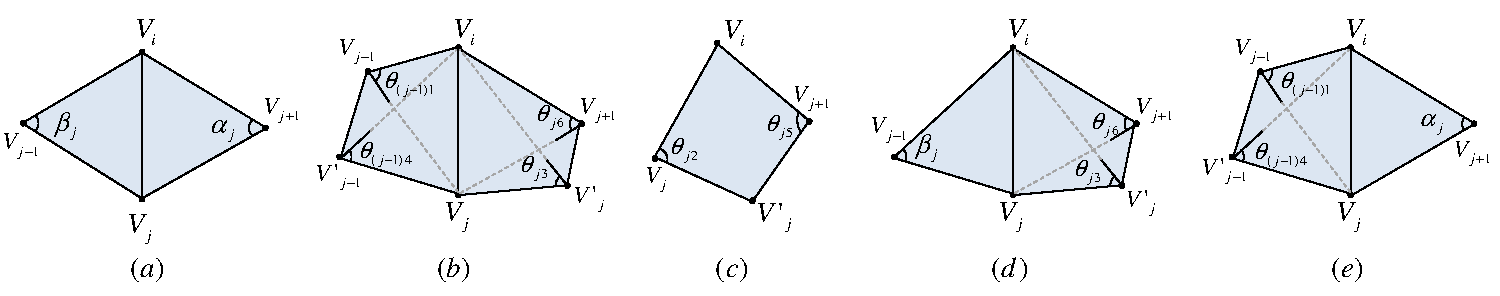
\includegraphics[width=1\textwidth]{images/beltrami}

\caption{\label{fig:LBO-basic-5-TQ}The 5 basic triangle-quad cases with common
vertex $V_{i}$ and the relationship with $V_{j}$ and $V_{j}^{\prime}$.
(a) Two triangles {[}Desbrun 1999{]}. (b) (c) Two quads and one quad
{[}Xiong 2011{]}. (d) (e) Triangles and quads (TQLBO).}
\end{figure*}


Computer graphics objects which have been reconstructed from real
world, contain undesirable noise. Laplacian Smooth techniques allow
noise reduction on a mesh's surface with minimal changes on its shape
while still preserves desirable geometry as well as the shape of the
original model. 

The functional used in many Laplacian smoothing approaches to constrain
energy minimization is based on a total curvature of a surface $S$.

\begin{equation}
E\left(S\right)=\int_{S}\kappa_{1}^{2}+\kappa_{2}^{2}dS\label{eq:total_cuarvature_integral}
\end{equation}


Where $\kappa_{1}$ and $\kappa_{2}$ are the two principal curvatures
of the surface $S$.


\subsection{Gradient of Voronoi Area}

\begin{figure}[h]
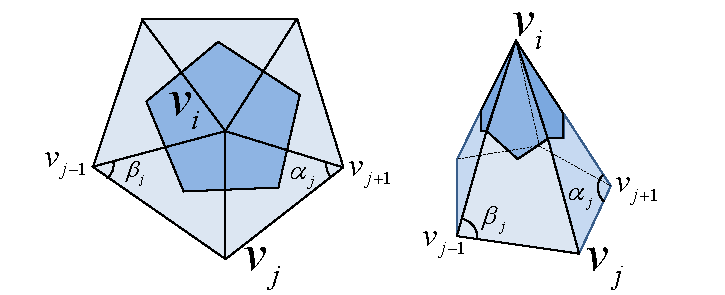
\includegraphics[width=1\columnwidth]{images/voronoi_region}

\caption{\label{fig:voronoi_region}Area of Voronoi region around $v_{i}$
in dark blue.\protect \\
 $v_{j}$ 1-ring neighbors around $v_{i}$. $\alpha_{j}$ and $\beta_{j}$
opposite angles to edge $\protect\overrightarrow{v_{j}-v_{i}}$. }
\end{figure}


Consider a surface $S$ composed by a set of triangles around vertex
$v_{i}$. We can define the \textit{Voronoi region} of $v_{i}$ as
show in figure \ref{fig:voronoi_region}, The change in the area produced
by the movement of $v_{i}$ is named gradient of \textit{Voronoi region
\cite{Pinkall1993,Desbrun1999,Meyer2003}.}

\begin{equation}
\nabla A=\frac{1}{2}\underset{j}{\sum}\left(\cot\alpha_{j}+\cot\beta_{j}\right)\left(v_{i}-v_{j}\right)\label{eq:eq_gradient_voronoi_area}
\end{equation}


If we normalize this gradient in equation (\ref{eq:eq_gradient_voronoi_area})
by the total area in 1-ring around $v_{i}$, we have the \textit{discrete
mean curvature normal} of a surface $S$ as shown in equation (\ref{eq:discrete_mean_curvature_normal}).

\begin{equation}
2\kappa\mathbf{n}=\frac{\nabla A}{A}\label{eq:discrete_mean_curvature_normal}
\end{equation}



\subsection{Laplace Beltrami Operator}

The \textit{Laplace Beltrami operator} LBO denoted $\triangle_{g}$
is used for measures mean curvature normal of the Surface $S$ \cite{Pinkall1993}. 

\begin{equation}
\triangle_{g}S=2\kappa\mathbf{n}\label{eq:def_LBO}
\end{equation}


The LBO has desirable features: one feature of the LBO is in direction
of surface area minimization, allowing to minimize energy using it
on a total curvature of a surface $S$ at equation (\ref{eq:total_cuarvature_integral}).


\section{Proposed Method\label{sec:Proposed-Method}}

Our method allows the editing of geometric features using the curvature
enhancement and smoothing, generating a parameterized family of shapes
from a set of vertices which represent a coarse sketch of the desired
model. Our approach can be mixed with traditional or uniform subdivision
surfaces methods, is iterative and converges towards a continuous
and smooth version of the original model. 

Unlike other methods, our method allows to use mixed arbitrary types
of mesh representation as triangles and quads, exploiting the basic
geometrical relationships facilitating and ensuring convergence of
the algorithm and similar shapes consistent with the original shape
against the other methods. 

Our method allows the use of soft constraints weighting the effect
of smoothing at each vertex based on a normalized weight, which are
assigned to the control vertices of the original mesh or. The weights
of the new vertices resulting from the subdivisions are calculated
by interpolation, allowing modifying the behavior of the method on
specific regions of the original model.

Our approach is based on an extension of the Laplace Beltrami operator
for meshes composed by triangles and quads. Interest on meshes composed
by triangles and quads has increasing in recent years due to the flexibility
of modeling tools as Blender 3D \cite{blender}. Today many artists
manually connect vertices such that its edition allows a simple way
to perform animation processes and interpolation \cite{Mullen2007}.
For these reasons it is very important to develop an operator that
allows working with this type of mesh immediately, eliminating the
need to preprocessing the mesh to convert to triangles and losing
the original design made by users.


\subsection{Laplace Beltrami Operator for Hybrid Quad/Triangle Meshes TQLBO\label{sub:Laplace-Beltrami-operator}}

Given a mesh $M=\left(V,Q,T\right)$, with vertices $V$, quads $Q$,
triangles $T$.

The area of $1$-ring neighborhood ($N_{1}$) with shared face quad
or triangle to vertex $v_{i}$ in $M$ is.

\begin{center}
$A\left(v_{i}\right)=A\left(Q_{N_{1}\left(v_{i}\right)}\right)+A\left(T_{N_{1}\left(v_{i}\right)}\right)$.
\par\end{center}

\begin{figure}[h]
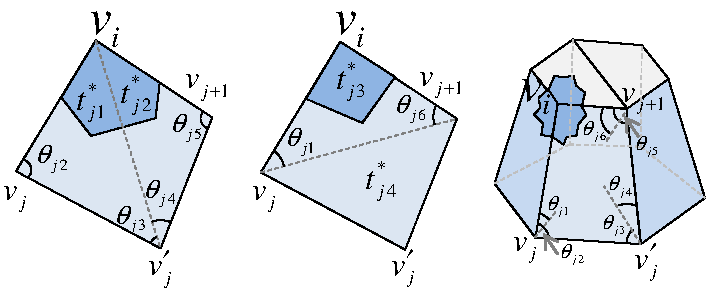
\includegraphics[width=1\columnwidth]{images/quad_xiong}

\caption{\label{fig:quad_xiong}$t_{j1}^{*}\equiv\vartriangle v_{i}v_{j}v_{j}^{\prime},\, t_{j2}^{*}\equiv\vartriangle v_{i}v_{j}^{\prime}v_{j+1},\, t_{j3}^{*}\equiv\vartriangle v_{i}v_{j}v_{j+1}$
Triangulations of the quad with common vertex $v_{i}$ proposed by
{[}Xiong 2011{]} to define Mean LBO.}
\end{figure}


Applying the mean average area according to \cite{Xiong2011} of all
possible triangulations for each quad to $A\left(Q_{N_{1}\left(v_{i}\right)}\right)$
as show in figure \ref{fig:quad_xiong}.

\begin{center}
$A\left(v_{i}\right)=\frac{1}{2^{m}}\overset{m}{\underset{j=1}{\sum}}2^{m-1}A\left(q_{j}\right)+\overset{r}{\underset{k=1}{\sum}}A\left(t_{k}\right)$
\par\end{center}

Where $q_{1},q_{2},...,q_{j},...,q_{m}\in Q_{N_{1}\left(v_{i}\right)}$
and $t_{1},t_{2},...,t_{k},...,t_{r}\in T_{N_{1}\left(v_{i}\right)}$.

\begin{equation}
A\left(v_{i}\right)=\frac{1}{2}\overset{m}{\underset{j=1}{\sum}}\left[A\left(t_{j1}^{*}\right)+A\left(t_{j2}^{*}\right)+A\left(t_{j3}^{*}\right)\right]+\overset{r}{\underset{k=1}{\sum}}A\left(t_{k}\right)\label{eq:area_1_ring_triangles_quads}
\end{equation}


Applying the gradient operator to (\ref{eq:area_1_ring_triangles_quads}).

\begin{equation}
\nabla A\left(v_{i}\right)=\frac{1}{2}\overset{m}{\underset{j=1}{\sum}}\left[\nabla A\left(t_{j1}^{*}\right)+\nabla A\left(t_{j2}^{*}\right)+\nabla A\left(t_{j3}^{*}\right)\right]+\overset{r}{\underset{k=1}{\sum}}\nabla A\left(t_{k}\right)\label{eq:EqGrad}
\end{equation}


According to (\ref{eq:eq_gradient_voronoi_area}), we have.

\begin{center}
$\nabla A\left(t_{j1}^{*}\right)=\frac{\cot\theta_{j3}\left(v_{j}-v_{i}\right)+\cot\theta_{j2}\left(v_{j}^{\prime}-v_{i}\right)}{2}$
\par\end{center}

\begin{center}
$\nabla A\left(t_{j2}^{*}\right)=\frac{\cot\theta_{j5}\left(v_{j}^{\prime}-v_{i}\right)+\cot\theta_{j4}\left(v_{j+1}-v_{i}\right)}{2}$
\par\end{center}

\begin{center}
$\nabla A\left(t_{j3}^{*}\right)=\frac{\cot\theta_{j6}\left(v_{j}-v_{i}\right)+\cot\theta_{j1}\left(v_{j+1}-v_{i}\right)}{2}$
\par\end{center}

\begin{center}
$\nabla A\left(t_{k}\right)=\frac{\cot\alpha_{k}\left(v_{k}-v_{i}\right)+\cot\beta_{k+1}\left(v_{k+1}-v_{i}\right)}{2}$
\par\end{center}

Thus triangles and quads configurations of the 1-ring neighborhood
faces adjacent to $v_{i}$ can be simplified to five cases shown in
figure \ref{fig:LBO-basic-5-TQ}.

Then according to equation (\ref{eq:discrete_mean_curvature_normal}),
(\ref{eq:def_LBO}), and five simple cases defined in figure \ref{fig:LBO-basic-5-TQ}
the TQLBO (Triangle-Quad LBO) of $v_{i}$ is.

\begin{equation}
\triangle_{g}\left(v_{i}\right)=2\kappa\mathbf{n}=\frac{\nabla A}{A}=\underset{v_{j}\in N_{1}\left(v_{i}\right)}{\frac{1}{2A}\sum}w_{ij}\left(v_{j}-v_{i}\right)
\end{equation}


\begin{equation}
w_{ij}=\begin{cases}
\left(\cot\alpha_{j}+\cot\beta_{j}\right) & \mbox{case }\mathit{a.}\\
\frac{1}{2}\left(\cot\theta_{\left(j-1\right)1}+\cot\theta_{\left(j-1\right)4}+\cot\theta_{j3}+\cot\theta_{j6}\right) & \mbox{case \ensuremath{\mathit{b}}.}\\
\left(\cot\theta_{j2}+\cot\theta_{j5}\right) & \mbox{case \ensuremath{\mathit{c}}.}\\
\frac{1}{2}\left(\cot\theta_{j3}+\cot\theta_{j6}\right)+\cot\beta_{j} & \mbox{case \ensuremath{\mathit{d}}.}\\
\frac{1}{2}\left(\cot\theta_{\left(j-1\right)1}+\cot\theta_{\left(j-1\right)4}\right)+\cot\alpha_{j} & \mbox{case \ensuremath{\mathit{e}}.}
\end{cases}\label{eq:TQLBO_wij}
\end{equation}


We define a Laplacian operator as a matrix equation

\begin{equation}
L\left(i,j\right)=\begin{cases}
-\frac{1}{2A_{i}}w_{ij} & \mbox{if }j\in N\left(v_{i}\right)\\
\frac{1}{2A_{i}}\underset{j\in N\left(v_{i}\right)}{\sum}w_{ij} & \mbox{if }i=j\\
0 & \mbox{otherwise}
\end{cases}\label{eq:TQLBO_Simple_Matrix}
\end{equation}


Where $L$ is a $n\times n$ matrix, $n$ is the number of vertices
of a given mesh $M$, $w_{ij}$ is the TQLBO defined in equation (\ref{eq:TQLBO_wij}),
$N\left(v_{i}\right)$ is the 1-ring neighborhood with shared face
to $v_{i}$, $A_{i}$ is the ring area around $v_{i}$.

Normalized version of the TQLBO as a matrix equation

\begin{equation}
L\left(i,j\right)=\begin{cases}
-\frac{w_{ij}}{\underset{j\in N\left(v_{i}\right)}{\sum}w_{ij}} & \mbox{if }j\in N\left(v_{i}\right)\\
\delta_{ij} & \mbox{otherwise}
\end{cases}\label{eq:TQLBO-Normalized_Matrix}
\end{equation}


Where $\delta_{ij}$ being the Kronecker delta function.


\subsection{Curvature Enhancing\label{sub:Curvature-Enhancing}}

\begin{figure*}[t]
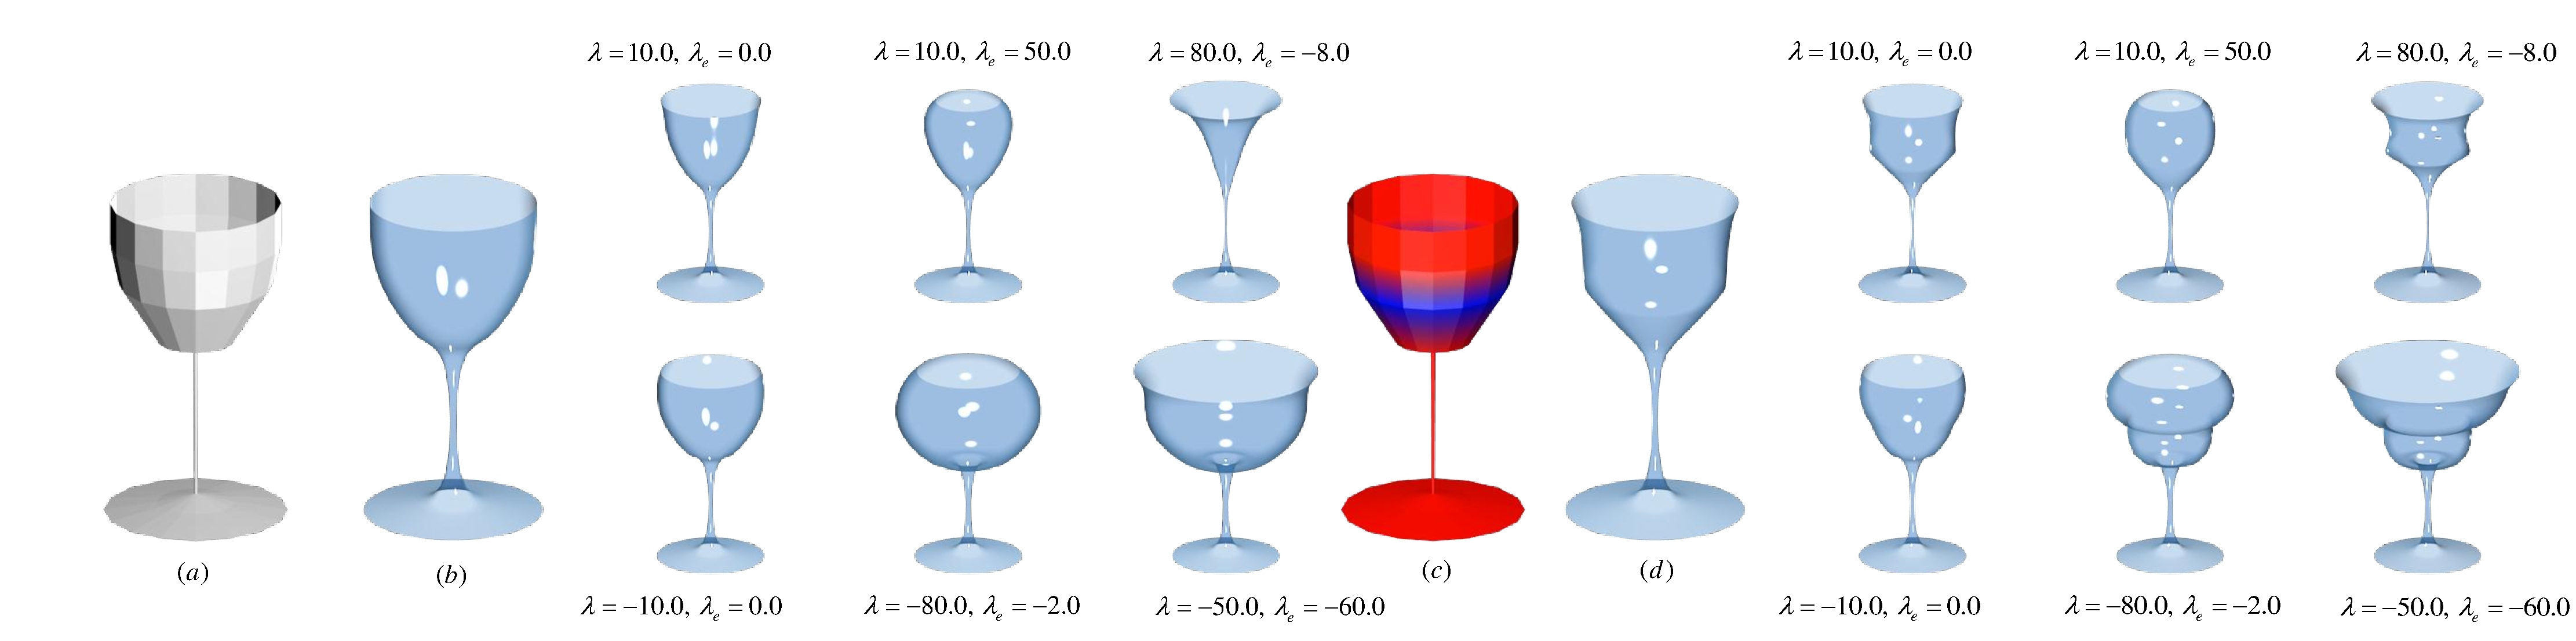
\includegraphics[width=1\textwidth]{images/teaser_cup}

\caption{\label{fig:Subdivision-Cups} Family of cups generated with our method
from coarse model to enhancing the curvature obtained from Catmull-Clark
Subdivision and the use of constraints over coarse model with weight
vertex group in red.}


\end{figure*}


The curvature enhancing uses the inverse direction of the curvature
flow to move the vertices in the portions of the mesh with most curvature.
In this equation we use a diffusion process:

\begin{center}
$\frac{\partial V}{\partial t}=\lambda L\left(V\right)$ 
\par\end{center}

To solve the equation above we use implicit integration and a normalized
version of TQLBO matrix.

\begin{equation}
\left(I-\left|\lambda dt\right|W_{p}L\right)V^{\prime}=V^{t}\label{eq:Lineal_System_with_wp}
\end{equation}


\begin{center}
$V^{t+1}=V^{t}+\mbox{sign}\left(\lambda\right)\left(V^{\prime}-V^{t}\right)$
\par\end{center}

The vertices $V^{t+1}$are enhanced along their inverse curvature
normal directions by solving the linear system: $Ax=b$, where $A=I-\left|\lambda dt\right|W_{p}L$,
$L$ is the Normalized TQLBO defined in the equation (\ref{eq:TQLBO-Normalized_Matrix}),
$x=V^{\prime}$ are the smoothing vertices, $b=V^{t}$ are the actual
vertices positions, $W_{p}$ is a diagonal matrix with weight vertex
group, and $\lambda dt$ is the enhance factor that support negative
and positive values, negative for enhancing positive for smoothing. 

The curvature cannot be calculted at the border of the meshes that
are not closed, for that reason we use the scale-dependent operator
proposed by \cite{Desbrun1999}.

Our method was designed for use with weighted vertex groups which
specify the final curvature enhancement on the solution, these weights
vary between $0$ and $1$ with a value of $0$ makes no changes and
with values 1 applies a maximal change. The weights modify influence
zones where the Laplacian is applied as shown in the equation \ref{eq:Lineal_System_with_wp}.
Families of shapes that are generated may change substantially with
the weights of specific control points.

The models volume increases as the lambda is larger and negative,
this can be go against by a simple method of volume preservation.
In \cite{Desbrun1999} presents a simple method to resize the mesh
however the model suffers large displacements when $\lambda<-1.0$
or after multiple iterations. We propose the following solution: If
$v_{i}^{t+1}$ is a mesh vertex of $V^{t+1}$ in the $t+1$ iteration,
we define $\overline{v}$ as:

\begin{center}
$\overline{v}=\frac{1}{n}\underset{v_{i}\in V}{\sum}v_{i}$, 
\par\end{center}

$\overline{v}$ is the center of the mesh, $vol_{ini}$ is an initial
volume, and $vol_{t+1}$ is the volume at the iteration $t+1$, then
we define a scale factor.

\begin{center}
$\beta=\left(\frac{vol_{ini}}{vol_{t+1}}\right)^{\frac{1}{3}}$
\par\end{center}

The new vertices positions are:

\begin{center}
$v_{i\, new}^{t+1}=\beta\left(v_{i}^{t+1}-\overline{v}\right)+\overline{v}$
\par\end{center}


\subsection{Sculpting\label{sub:Sculpting}}

\begin{figure*}[t]
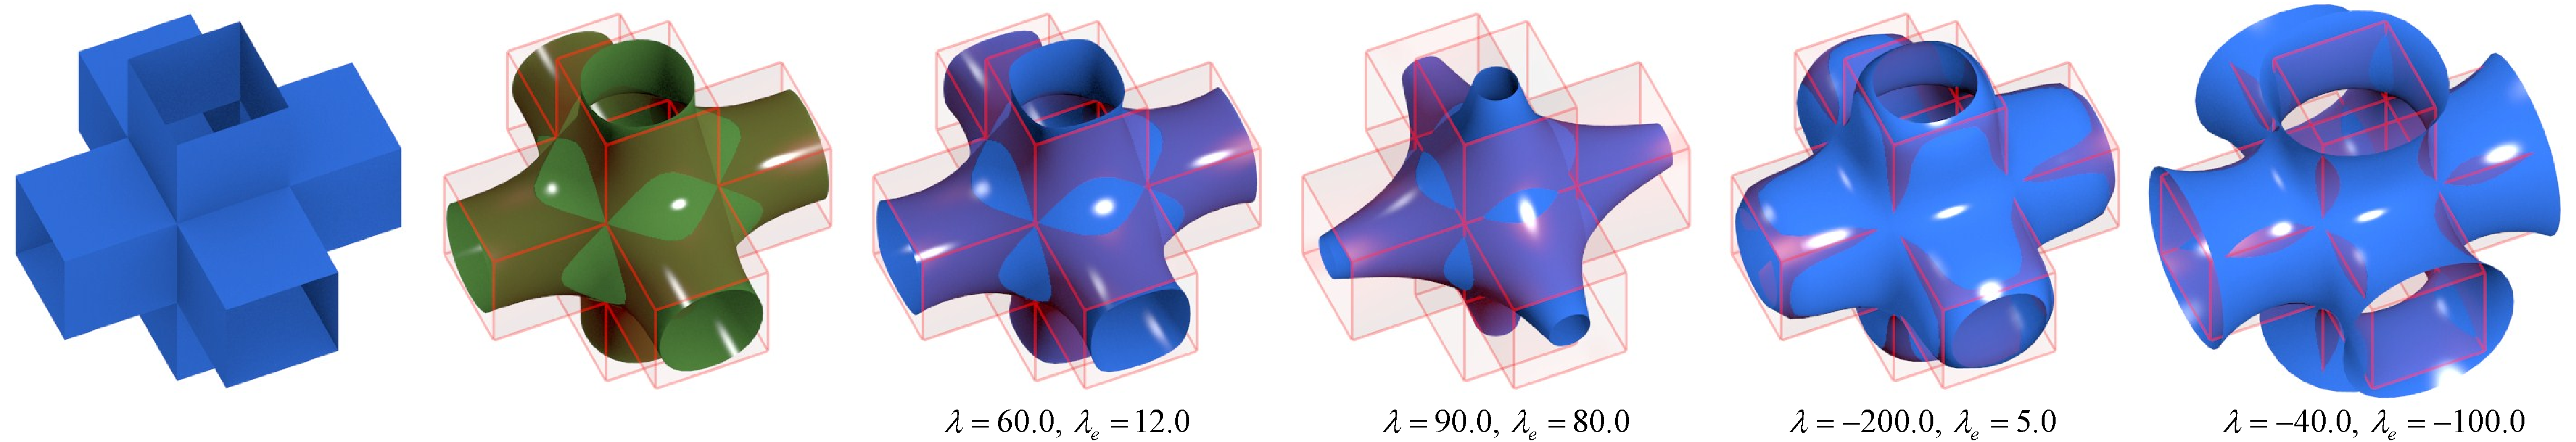
\includegraphics[width=1\textwidth]{images/cruz_lambda4}

\caption{\label{fig:Catmull_Clark}Left: Original Model, in green color model
with Catmull-Clark Subdivision. Models with Laplacian smoothing: $\lambda=60.0$,
$\lambda_{e}=12.0$ and $\lambda=90.0$, $\lambda_{e}=80.0$. Models
first filter with Laplacian smoothing $\lambda=60.0$, $\lambda_{e}=12.0$
and before applied curvature enhancing: $\lambda=-200.0$, $\lambda_{e}=12.0$
and $\lambda=-40.0$, $\lambda_{e}=-100.0$.}
\end{figure*}


We designed a new brush that allows the enhancement of the curvatures
of a polygon mesh in real time. Our brush works well with the stroke
method named \textsl{Drag Dot}  which allows to preview the changes
in the model before you release the mouse button or pen tablet, also
allows to move the mouse over the model to fit exactly where you want
to perform the enhancement of the curvature.

Brushes that perform similar work as inflate can create distortions
in the mesh and can also produce self-intersections in the mesh, as
these brushes only move the vertices along the normal and do not take
into account the global information. Whereas our method looks for
the best way to make inflation while preserving the global curvature
retaining the several shape and sharp features of the model.

Our method simplifies the work required for the enhancement, which
would be to use some different brushes for inflating and some other
to soften and styling. With our enhanced brush in one step can be
performed.

For the real-time brush it necessary that the Laplacian matrix is
constructed with the vertices that are within the radius  of the sphere
defined by the user, which reduces the size of the matrix to be processed,
the center of this sphere depends on the place where the user clicks
on the canvas and three-dimensional mesh place where the click is
projected. 

Furthermore special handling is required for the vertices at the boundary
which have neighbors that are not within the radius of the brush.
These vertices must be marked as boundary and the curvature will not
be calculated for them, but must be present in the matrix so that
every vertex has their neighbors within the selection, this change
allows the results to be much smoother on the border. The Laplacian
matrix for sculpt mode as a matrix equation.

\begin{center}
$L\left(i,j\right)=\begin{cases}
-\frac{w_{ij}}{\underset{j\in N\left(v_{i}\right)}{\sum}w_{ij}} & \mbox{if }\left\Vert v_{i}-u\right\Vert <r\wedge\left\Vert v_{j}-u\right\Vert <r\\
0 & \mbox{if }\left\Vert v_{i}-u\right\Vert <r\wedge\left\Vert v_{j}-u\right\Vert \geq r\\
\delta_{ij} & \mbox{otherwise}
\end{cases}$
\par\end{center}

Where $v_{j}\in N\left(v_{i}\right)$, $u$ is the center of sphere
of radius $r$. The matrixes should remove rows and columns of vertices
index that are not within the radius.


\subsection{Subdivision surfaces\label{sub:Subdivision-surfaces}}

The Catmull-Clark subdivision transformation is used to smooth a surface
as the limit of a sequence of subdivision steps\cite{Stam1998}. This
process is governed by properties of B-splines curve from multivariate
spline theory\cite{Loop1987}. This method does a recursive subdivision
transformation that refines the model into a linear interpolation
that approximates a smooth surface. The smoothness of the model is
automatically guaranteed \cite{DeRose1998}. 

Catmull-Clark subdivision surface methods generate smooth and continuous
models from a coarse model and produce results quickly due to the
simplicity of implementation, but with these methods is not easy to
make changes to the global curvature of the model. If we use Catmull-Clark
subdivision surfaces and curvature enhancement for modeling from coarse
models with few vertices can generate families of shapes changing
a single parameter, this would allow an artist to choose the model
from a similar set of options that best meets his/her needs without
having to change each one of the control vertices.

Our method allows the use of vertex weight paint over the control
points. The weights can be applied to a coarse model, then to perform
a Catmull-Clark subdivision where weights are interpolated, producing
weights with smooth changes in the zones of influence, so the obtained
curvature is much softer at those areas as shown in figure \ref{fig:Subdivision-Cups}.c.

In the equation \ref{eq:Lineal_System_with_wp}, $W_{p}$ is a diagonal
matrix with weights corresponding to each vertex. Weights at each
vertex produce a different solution for this reason the matrix is
placed in the diffusion equation, as families that are generated may
change substantially with weighted of specific control points.


\section{Results\label{sec:Results}}

In this section we describe the results of our curvature enhance method
with the extension of the Laplace Beltrami operator for hybrid quad/triangle
meshes with several example models (see figures \ref{fig:Spectrum},
\ref{fig:Subdivision-Cups}, \ref{fig:Catmull_Clark}, \ref{fig:TQLBO_test},
\ref{fig:camello_enhanced}, \ref{fig:Sculpt_Brush}, \ref{fig:Performance-sculpt},
\ref{fig:(a)Monkey}, \ref{fig:Animated_Camell}). We test the curvature
enhance with TQLBO method on a PC with AMD Quad-Core Processor @ 2.40
GHz and 8 GB RAM.

Figure \ref{fig:TQLBO_test} show the results when applying Laplace
Beltrami Operator TQLBO of equation (\ref{eq:TQLBO_Simple_Matrix})
in a model with a simple subdivision. In column (c) Laplacian smoothing
was applied to the model consists of only quads. In column (d) the
model was converted to triangles and then Laplacian smoothing was
applied. In column (e) the model is converted randomly some quads
into triangles and then Laplacian smoothing is applied, showing similar
results to those composed only of triangles or squares.

\begin{figure}
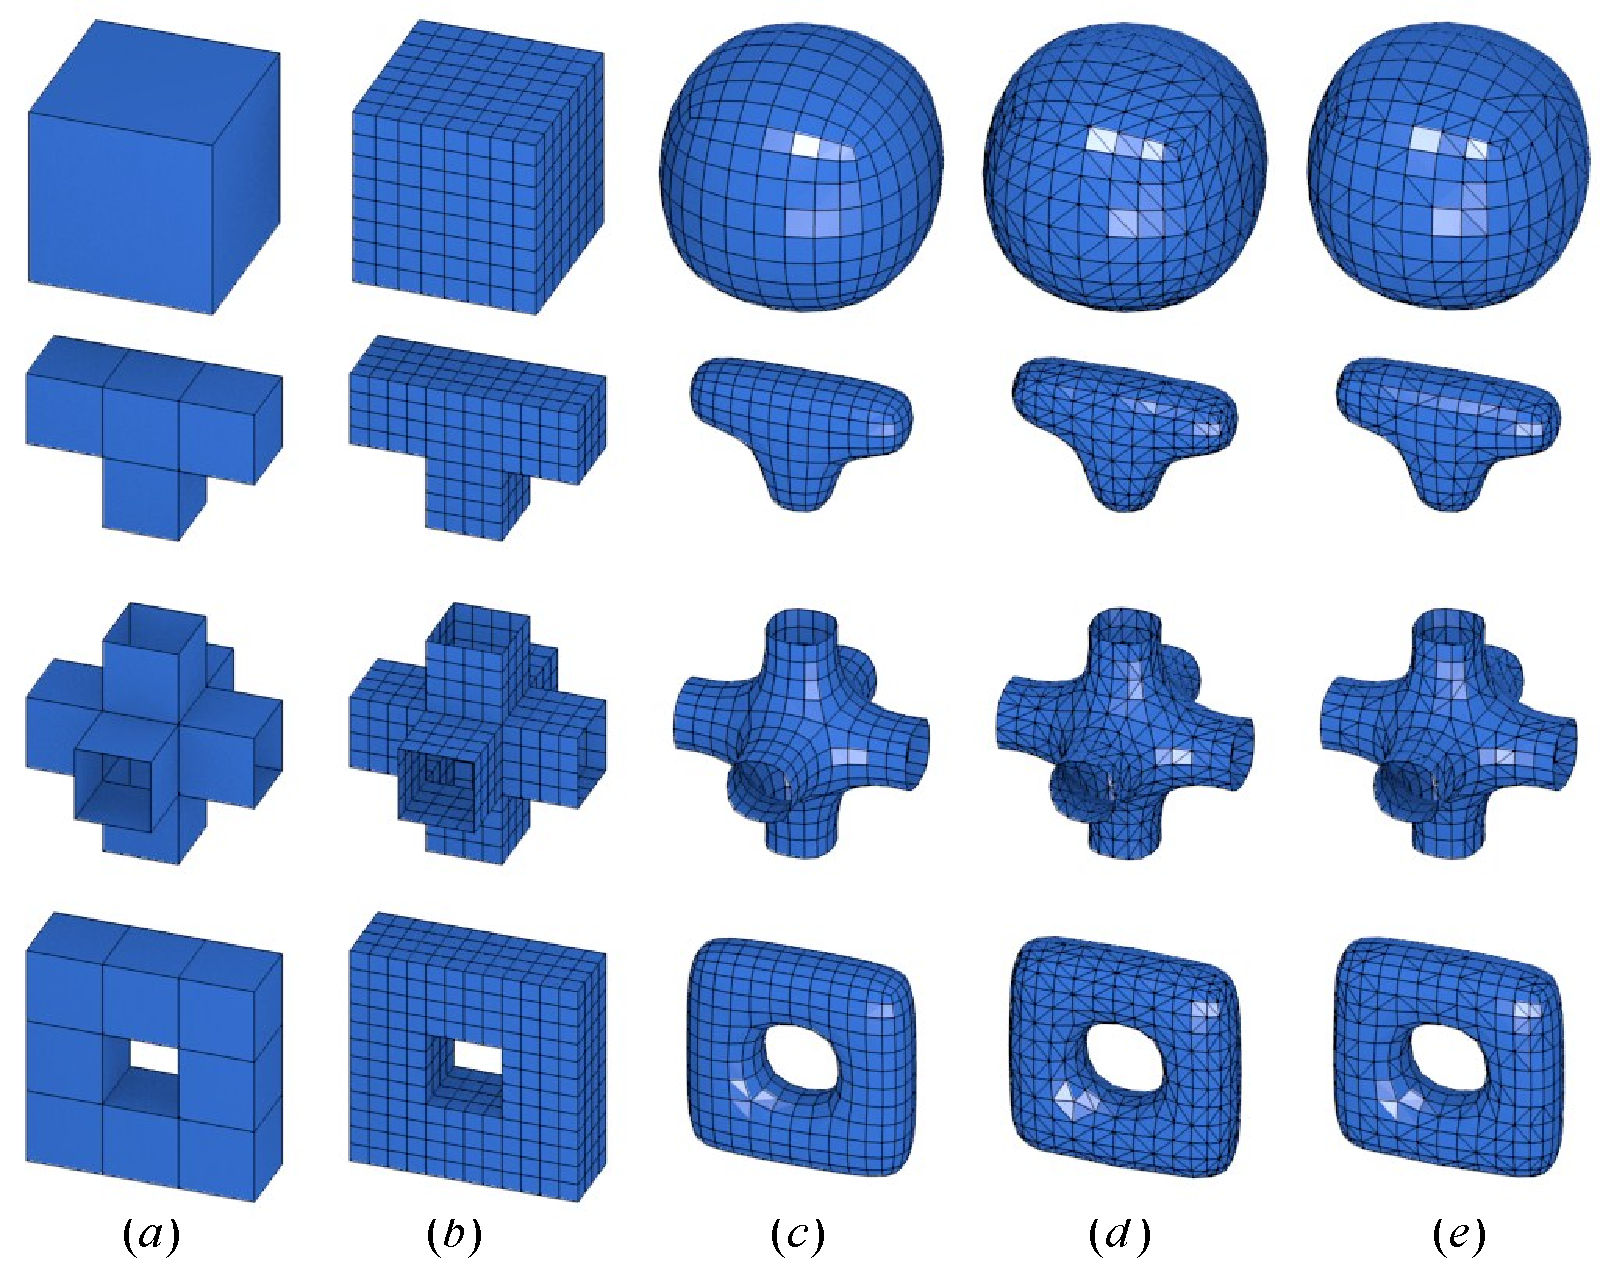
\includegraphics[width=1\columnwidth]{images/test_triangles_quads}

\caption{\label{fig:TQLBO_test}(a) Original Model. (b) Simple subdivision.
(c), (d) (e) Laplacian smoothing with $\lambda=7$ and 2 iterations:
(c) for triangles, (d) for quads, (e) for triangles and quads random
chosen.}
\end{figure}


Methods using Catmull-Clark subdivision surface and the enhancement
allows to modify the curvature that is obtained with the process of
subdivision as shown in figure \eqref{fig:Subdivision-Cups} this
test used a coarse model of a cup, after the model was performed subdivision
then was performed Laplacian smoothing and enhancement by modifying
the parameters $\lambda$ y $\lambda_{e}$ corresponding to the lambda
for rings and edges respectively. In figure \eqref{fig:Subdivision-Cups}.c,
\eqref{fig:Subdivision-Cups}.d shows also the use weight vertex groups
over coarse models with subdivision surfaces that allowed to generate
the weights for the new interpolated vertices, these new weights were
used for the enhancement obtained the 6 cups that are to the right
of the figure \eqref{fig:Subdivision-Cups}.d.

Laplacian smoothing applied with simple subdivision may produce similar
results to those obtained with Catmull-Clark whose models are on average
equal triangles as shown in figure \ref{fig:Catmull_Clark} green
model and that obtained with Laplacian smoothing $\lambda=60.0$,
$\lambda_{e}=12.0$, but also can modify the curvature obtained after
applying Catmull-Clark as shown in the three columns to the right
of the figure \ref{fig:Catmull_Clark}.

Figure \ref{fig:camello_enhanced} show the generation of different
versions of a camel according to parameter lambda. In the top row
you can see results of do curvature enhance over all model, as the
lambda becomes larger and negative in this model it inflates the convex
parts as shown in figure \ref{fig:Spectrum}. The larger $\lambda$
the larger enhancements on the model features. The bottom row of figure
\ref{fig:camello_enhanced} shows the use of weighted vertex groups,
which allows to specify which areas will be enhanced. On the left
the enhancement of the legs of the camel is shown which produces enhancement
of organic aspect, notice that the border is not distorted and smooth
in the union.

\begin{figure}
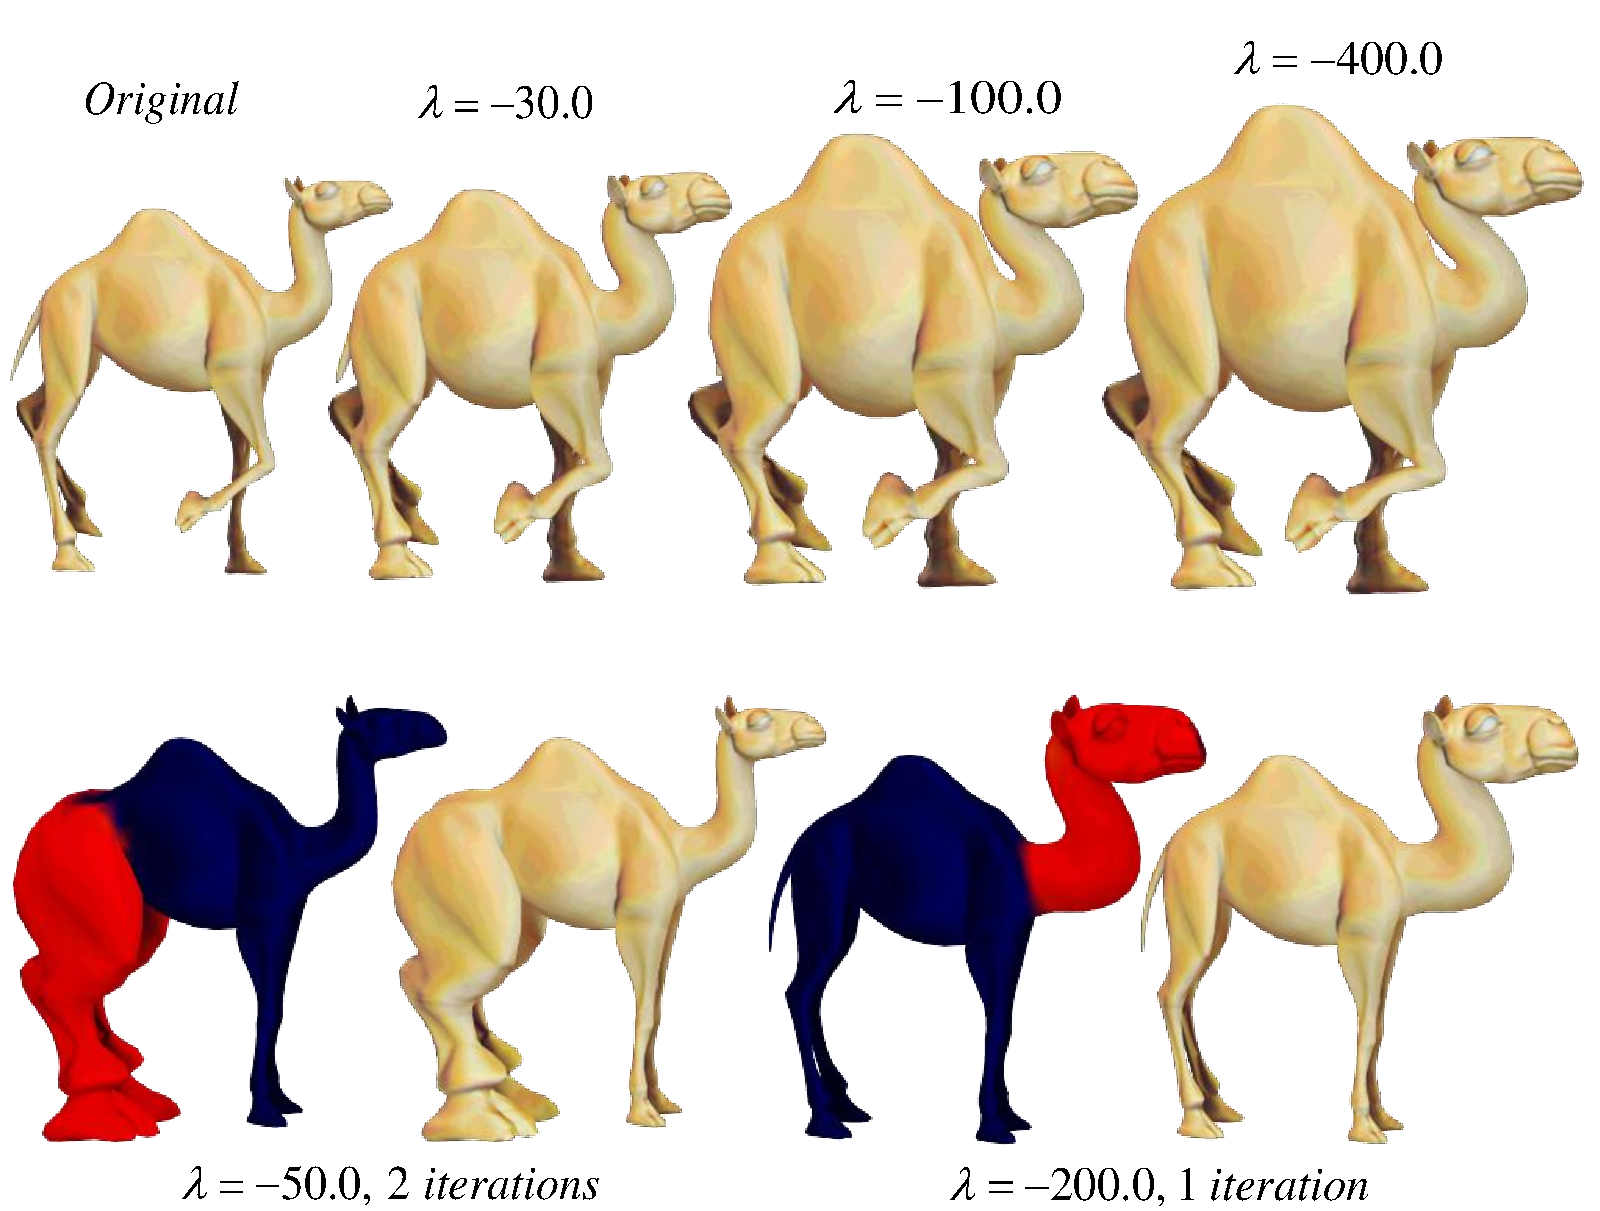
\includegraphics[width=1\columnwidth]{images/camello_enhanced2}

\caption{\label{fig:camello_enhanced}Top row: Original camel model in left.
Curvature enhancing with $\lambda=-30.0$, $\lambda=-100.0$, $\lambda=-400.0$.
Bottom row: Curvature enhancing with weight vertex group, $\lambda=-50.0$
and 2 iterations at legs, $\lambda=-200.0$ and 1 iteration in head
and neck.}
\end{figure}


Our method for enhancement of the silhouette features is predictable
and invariant under isometric transformations as those present in
some animations (see Figure \ref{fig:Animated_Camell}). This animation
shows some poses of a camel during a walk, enhancement is performed
in the neck and legs as shown in the bottom left part of the figure
\ref{fig:Animated_Camell}. Local modifications produced by pose interpolation
or animation rigging do not significantly affect the result as with
camel legs in each sample pose different flexion of the leg joints
enhancement camel keeps flesh-like shapes in the pattern produced
original by the artist. This is due to the diffusion process which
is subjected to the mesh so that small local changes are treated without
significantly affecting global solution. Our method is invariant of
rotation, this since depends exclusively on the normal field of the
mesh, wish is invariant under global rotations. 

Figure \ref{fig:Sculpt_Brush} shows the use of curvature enhancement
brush for sculpting in real time. One pass was used with the brush
as shown in the figure with the blue and red radius. In figure \ref{fig:Sculpt_Brush}.b
camel shows how the leg self-intersecting and looks like two bubbles
stuck, the same happens to the fingers on the bottom of the figure.
Using silhouette features enhancement in figure \ref{fig:Sculpt_Brush}.c
we get better results sd the are retained shape of the silhouette
and the details of the fingers and leg. Similar results can be obtained
by an artist however it would take several steps and require the use
of several brushes. With curvature enhancement it only takes one step.
This new method can easily enhance organic features like muscles during
the sculpting process. In figure \ref{fig:Performance-sculpt} we
show the performance of curvature enhancement brush, in this experiment
we use three models with 12K, 40K and 164K vertices, this models were
sculpted with curvature enhance brush in each step the brush sphere
contain a variable number of vertices for processing. The processing
time for 800 vertices in the camel paw (40k model) only take 0.1 seconds,
for 2600 vertices in leg and neck (model 40k) take 0.5 seconds, these
times are good, because usually an artist sculpts a model for parts,
and each part is represented by an average of about 3000 vertices
in the models we use.

Tests with the Laplacian operator equation (\ref{eq:TQLBO_Simple_Matrix})
and its normalized version equation (\ref{eq:TQLBO-Normalized_Matrix}),
produce similar results if the triangles that compose the mesh are
the same size on average. The normalized version is more stable and
predictable because it is not divided by the area of the ring which
may be very small and cause problems during floating point calculations
as shown in figure \ref{fig:(a)Monkey}.c bottom row. The enhancement
of curvature of the model with the normalized Laplacian operator has
a more regular behavior. The model can be deformed in TQLBO normalized
version with large lambdas ($\lambda>400$) while it intersects itself
it produces no peaks. Figure \ref{fig:(a)Monkey} shows different
results due to the area of the triangles in the model. Triangles with
larger area have smaller enhancement (figure \ref{fig:(a)Monkey}.c
skull), and smaller triangles have larger enhancements (figure \ref{fig:(a)Monkey}.c
chin).

\begin{figure}
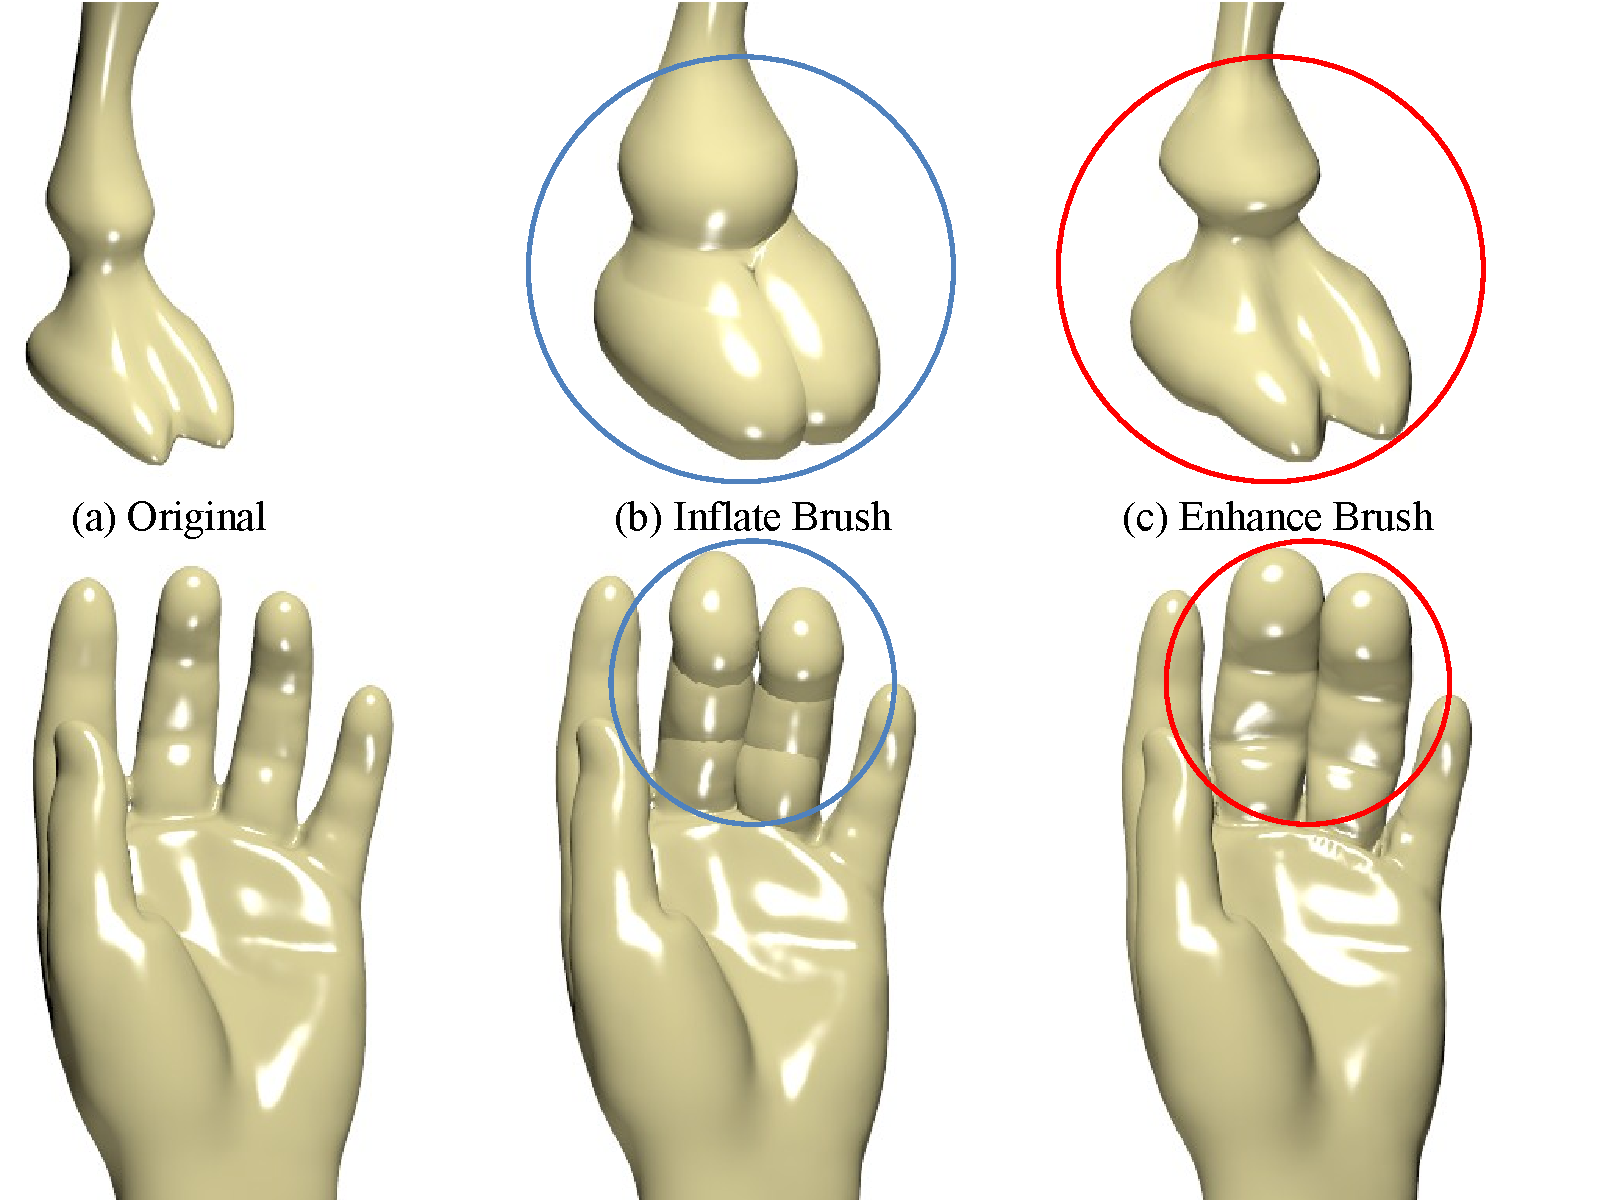
\includegraphics[width=1\columnwidth]{images/sculpt_brush}

\caption{\label{fig:Sculpt_Brush}Top row: (a) Leg Camel, (b) Inflate brush
for leg into blue circle, (c) Enhance curvature brush for leg into
red circle. Bottom row: (a) Hand, (b) Inflate brush for fingers into
blue circle, (c) Enhance curvature brush for fingers in red circle.}
\end{figure}


\begin{figure}
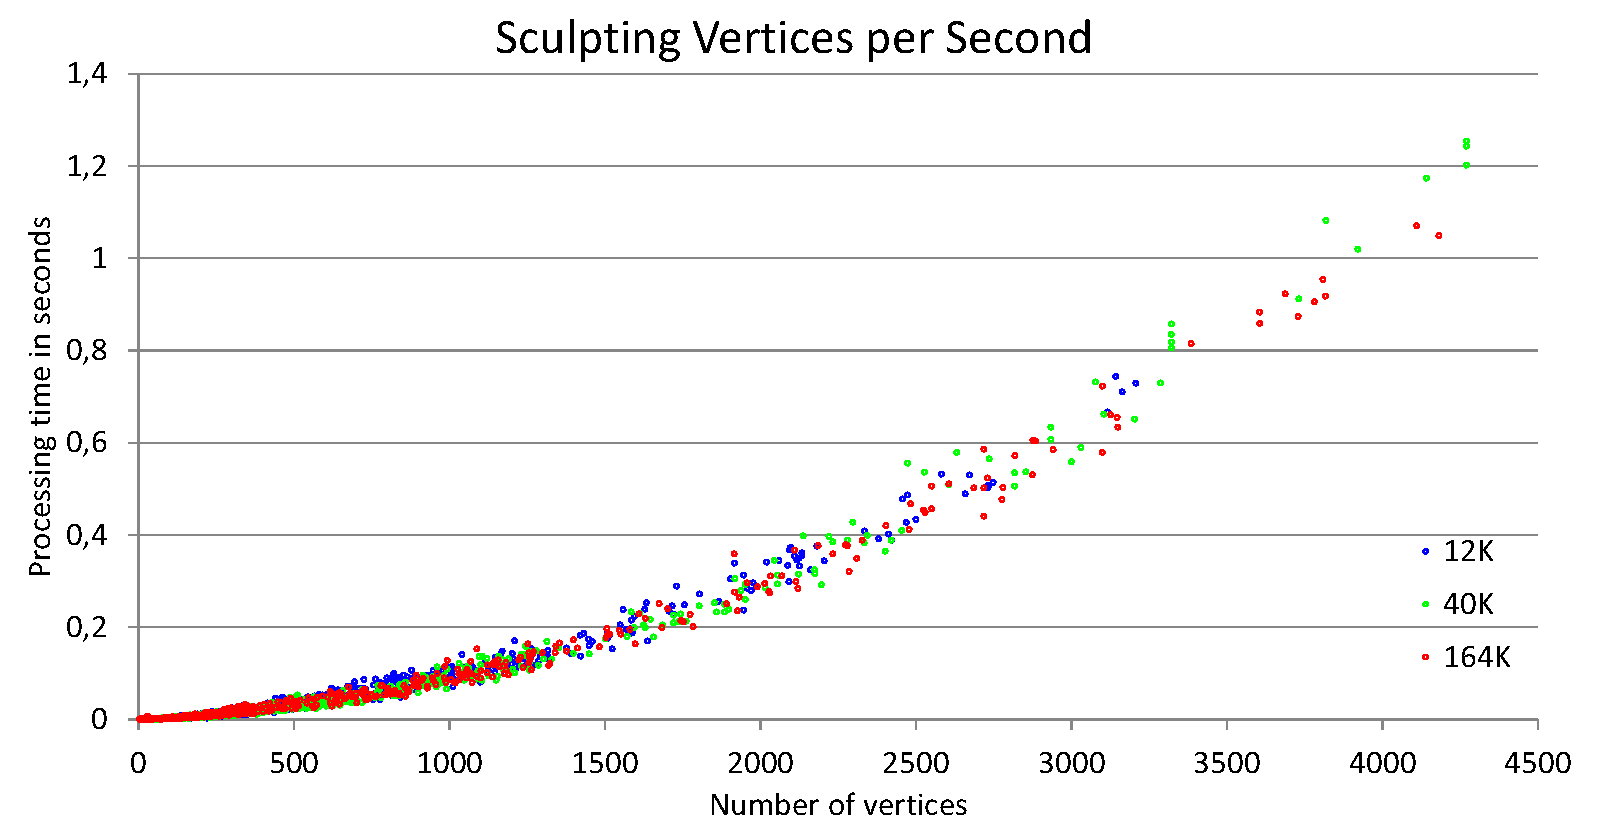
\includegraphics[width=1\columnwidth]{images/verts_per_second_sculpt}

\caption{\label{fig:Performance-sculpt}Performance of our dynamic curvature
enhance brush in terms of vertices sculpted per second. Three models
with 12K, 40K, 164K vertices used for sculpting in real time.}
\end{figure}


\begin{figure}
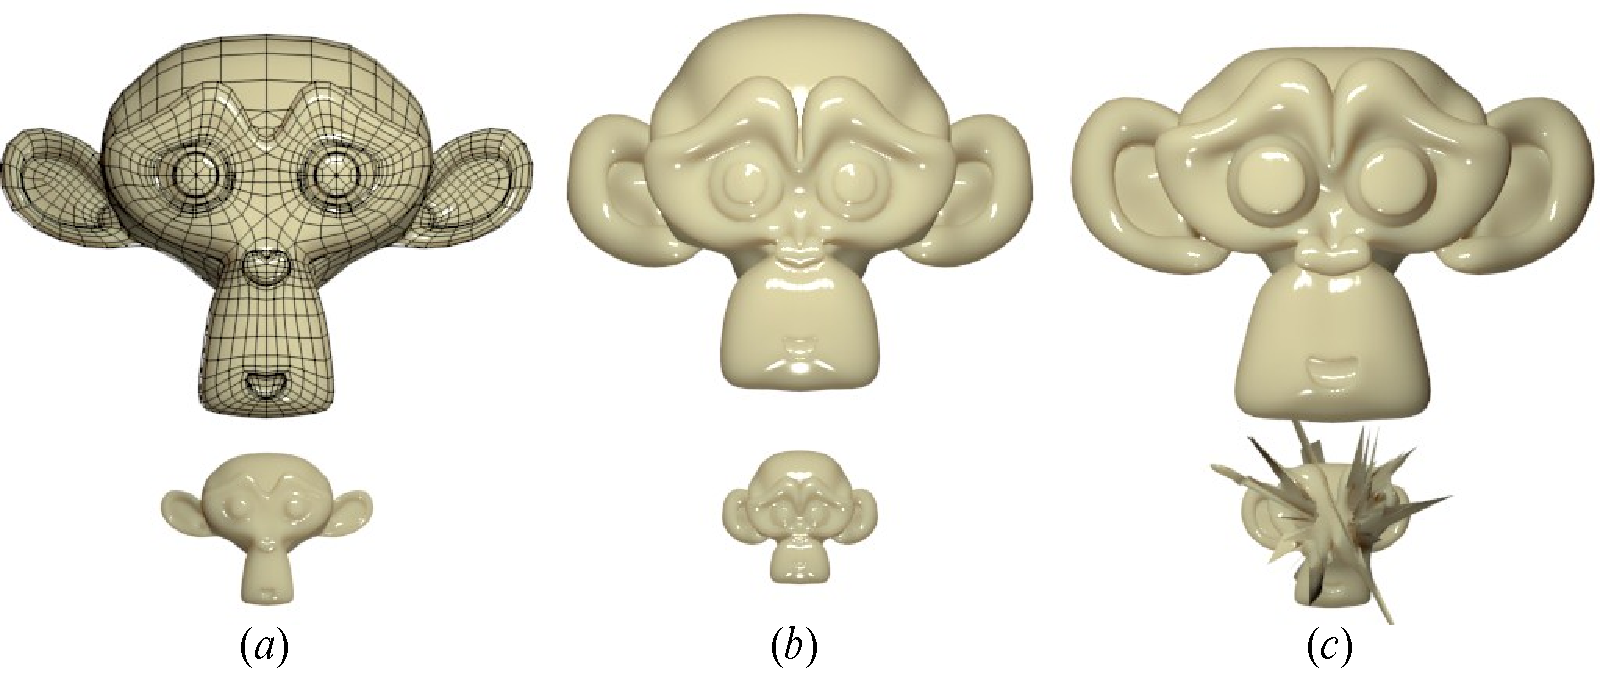
\includegraphics[width=1\columnwidth]{images/monkey}

\caption{\label{fig:(a)Monkey}(a) Top row: Original model scaled by 4. Bottom
row: Original Model (b) Top and bottom row: enhancing with Normalized-TQLBO
$\lambda=-50$ (c) Top and bottom row: enhancing with TQLBO $\lambda=-50$.}
\end{figure}


\begin{figure*}[t]
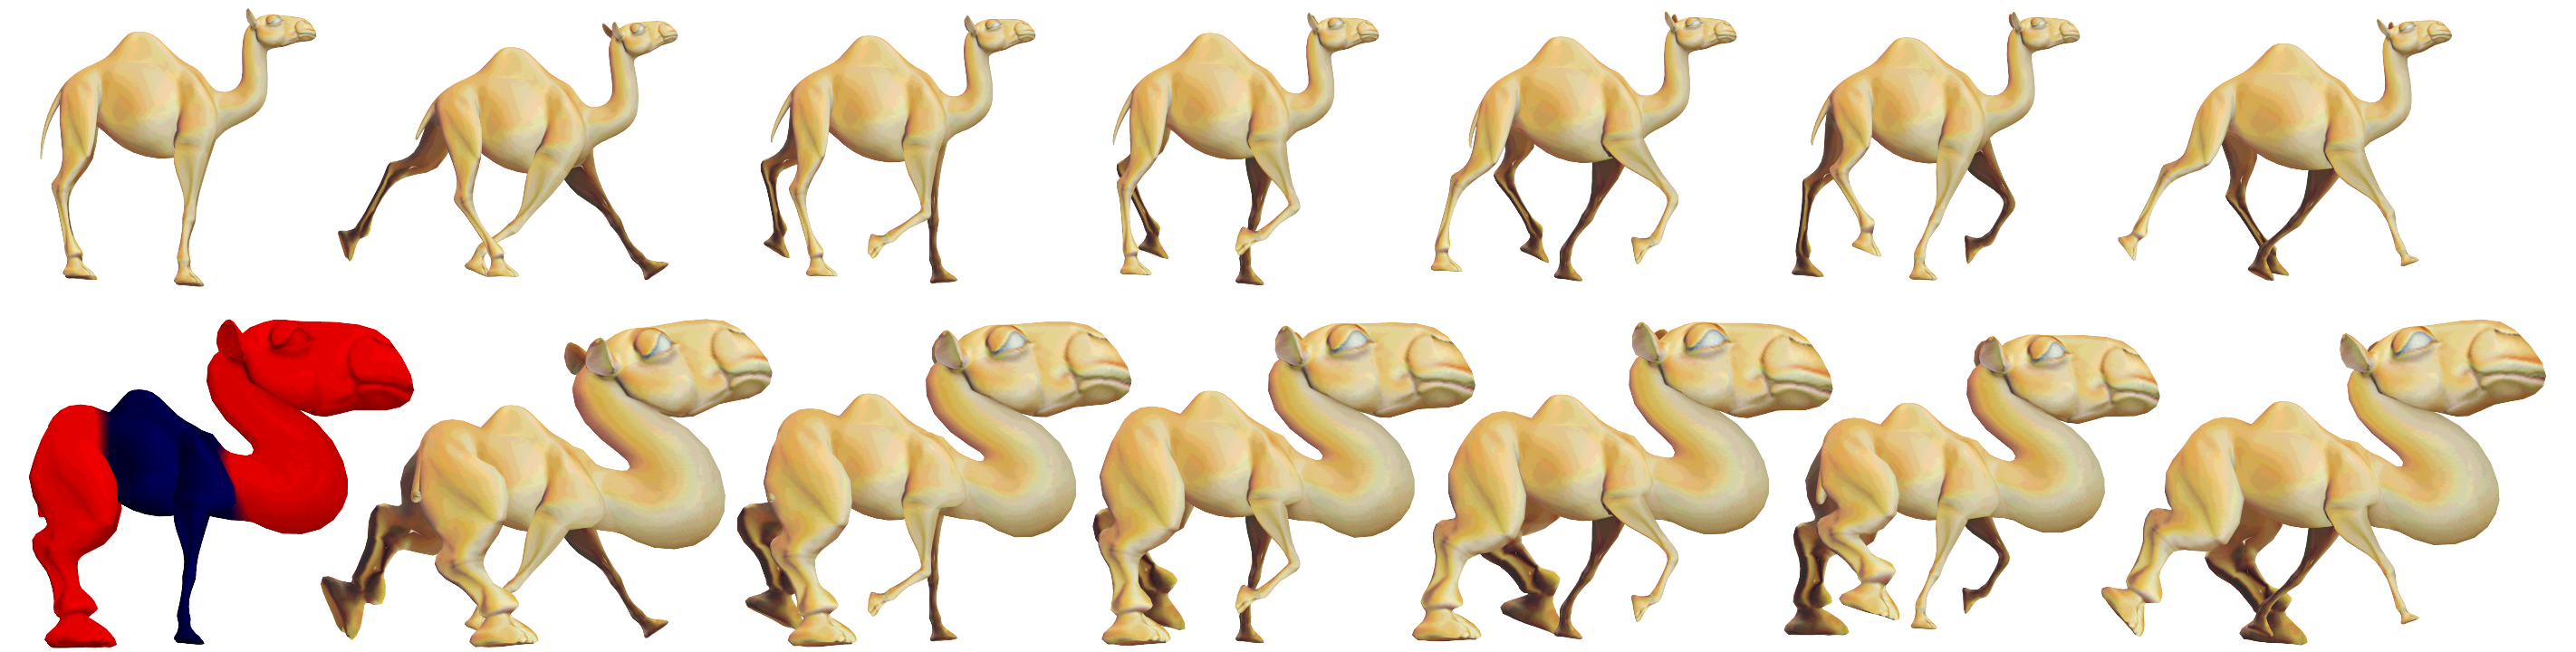
\includegraphics[width=1\textwidth]{images/camello_walk2}

\caption{\label{fig:Animated_Camell}Our method is pose insensitive. The enhanced
for the different poses are similar in terms of shape. Top row: Original
walk cycle camel model. Bottom row: Curvature enhancing with weight
vertex group, $\lambda=-400$ and $2$ iterations. }
\end{figure*}



\subsection{Implementation\label{sub:Implementation}}

Our method was implemented as a modifier for modeling and brush for
sculpting on the Blender software \cite{blender} with C and C++.
Working with Blender allowed us to test the method interactively against
others as Catmull-Clark, weight vertex groups and sculpting system
in Blender.

To improve the performance, we worked with Blender mesh struct visiting
each triangle or quad and adding its corresponding index in a list
that stores the sum of the Laplacian weights of the ring, in this
way we only had to visit two times the list of faces of the mesh list
and two times the list of the edges if the mesh was not closed. The
brush sculpting mode required to create a list that maps the index
of the selected vertices to a list from 1 to N where N is the number
of vertices selected and the number of rows in the linear system to
solve. This drastically reduced the calculations enabling real-time
processing. In the construction of our Laplacian matrix several index
were locked at vertices having faces areas or lengths edges with value
zero that can cause spikes and bad results.

Under this conditions matrix at the equation\ref{eq:TQLBO_Simple_Matrix}
is sparse since the number of neighbors per vertex corresponding to
the number of data per row is small compared to the total number of
vertices in the mesh. To solve the linear system equation \ref{eq:Lineal_System_with_wp}
was used OpenNL which is a a library for solving sparse linear system.


\section{Conclusion and future work\label{sec:Conclusion-and-future}}

This work presented an extension of the Laplace Beltrami operator
for hybrid quad/triangle meshes that can be used in production environments
without modification that provides results similar to those obtained
by working only with triangles or quads. 

We introduced a new way to perform silhouettes enhancement in a mesh
for modeling or sculpting in a few steps which allows the modification
of the curvature of a model while preserving its overall shape. We
introduce a new method of modeling and show some of its possible uses.
This method behaves in predictable ways which facilitate the learning
process, and works well with isometric transformations opening the
possibility of introducing it on the process of animation.

We show that this tool could work in the early stages in where coarse
models are used, allowing to modify the curvature generated by the
Catmull-Clark subdivision surfaces, avoiding the edition of the vertices
with the change of a few parameters.

As future work we analyze theoretically the relationship between the
Catmull-Clark subdivision surfaces and Laplacian smoothing because
in some cases can produce very similar results. But the subdivision
surface is a fast method thereby reducing computation times for calculate
curvature in the mesh.


\section*{Acknowledgments}

We wold like to thank  anonymous friends for their support of our
research. 

This work was supported in part by the Blender Foundation, Google
Summer of code program at 2012. 

Livingstone elephant model is provided courtesy of INRIA and ISTI
by the AIM@SHAPE Shape Repository. Hand model is courtesy of the FarField
Technology Ltd. Camel model by Valera Ivanov is licensed under a Creative
Commons Attribution 3.0 Unported License. Dinosaur and Monkey models
are under public domain, courtesy of Blender Foundation.

\bibliographystyle{acmsiggraph/acmsiggraph}
\bibliography{template}
 
\end{document}
